\documentclass{beamer}

\usepackage{color}
%\definecolor{class}{RGB}{111,159,207}
%\definecolor{literal}{rgb}{0.58,0,0.82}

\usepackage{hyperref}
\hypersetup{colorlinks=true, linkcolor=black, citecolor=blue, urlcolor=blue}

\usepackage[absolute,overlay]{textpos}
\TPGrid{100}{100}

\usepackage[ % BIBLATEX
  backend=bibtex,
  style=numeric-comp,sorting=none,block=ragged,firstinits=true
]{biblatex}
\bibliography{tilelvreqs}

\usepackage{tikz}

%\usepackage{forloop}
\usepackage{pdfpages}
\usepackage{pgf}

% Fixes ---------------------------------------------------
%\usepackage{lmodern}
\usepackage{silence}
\WarningFilter{biblatex}{Patching footnotes failed}

\let\Tiny=\tiny

% Slide styles --------------------------------------------
\setbeamersize{text margin left=20px,text margin right=20px}
\setbeamertemplate{navigation symbols}{}
\setbeamertemplate{section in toc}[sections numbered]
\setbeamertemplate{subsubsection in toc}[subsubsections numbered]
\setbeamertemplate{footline}{%
  \usebeamerfont{author in head/foot}%
  \insertshortauthor[width={1.7cm},respectlinebreaks,center]%
  \hspace*{-0.8mm},\ %
  \usebeamerfont{date in head/foot}\insertdate%
  \hspace*{1mm}%
  \usebeamerfont{footline}\url{https://indico.cern.ch/event/467725/}%
  \hfill%
  \insertframenumber/\inserttotalframenumber%
  \hspace*{1mm}
}
\setbeamertemplate{bibliography item}{\insertbiblabel}

\def\changemargin#1#2{\list{}{\rightmargin#2\leftmargin#1}\item[]}
\let\endchangemargin=\endlist

% Title, Authors, Date ************************************
\title{Low Voltage Monitoring Upgrade\\for ATLAS Tile Calorimeter}
\author[Ivan Pogrebnyak]
{%
  \texorpdfstring{
    \centering
    I. Pogrebnyak \\
    Working with: A. Paramonov, G. Drake, J. Proudfoot \\
  }{Ivan Pogrebnyak}
}
\date{December 8, 2015}

%%%%%%%%%%%%%%%%%%%%%%%%%%%%%%%%%%%%%%%%%%%%%%%%%%%%%%%%%%%
\begin{document}

% Title slide ---------------------------------------------
\frame{
  \begin{tikzpicture}[remember picture,overlay]
    \node[anchor=north west] at (current page.north west){
      \includegraphics[height=30pt]{logos/msu_helmet}
      \vspace{5px}
      \includegraphics[height=30pt]{logos/msu_text}
    };
    \node[anchor=north east] at (current page.north east){
      \begin{minipage}{100px}
      \vspace{-21px}
      {\huge Argonne}\\
      {\large National Laboratory}
      \end{minipage}
      \includegraphics[height=30pt]{logos/argonne_logo}
    };
    \node[anchor=south west] at (current page.south west){
      \begin{minipage}{100px}
      \includegraphics[height=30pt]{logos/DOE_Logo_Color}
      \vspace{8px}
      \end{minipage}
    };
    \node[anchor=south east] at (current page.south east){
      \begin{minipage}{96px}
      {\huge ATLAS}
      \vspace{-21px}\\
      {\large Experiment}
      \hspace{5px}
      \includegraphics[height=30pt]{logos/cern_logo}
      \vspace{8px}
      \end{minipage}
    };
  \end{tikzpicture}

  \titlepage
}

% TOC -----------------------------------------------------
\frame{\frametitle{Outline}\tableofcontents}

% *********************************************************

\setlength{\leftmargini}{2px}

\section{TileCal hardware and electronics}
\frame{\frametitle{Outline}\tableofcontents[currentsection]}

\frame{\frametitle{TileCal hardware}
  \begin{changemargin}{-20px}{-20px}
    \centering
    \includegraphics[width=0.9\textwidth]{fig/TileCal_barrels.jpg}
  \end{changemargin}
  \begin{textblock}{30}(7,83)
    LB - Long Barrel\\
    EB - Extended Barrel
  \end{textblock}
  \begin{textblock}{1}(88,90)
    {\tiny Ref.~\cite{twiki.ific}}
  \end{textblock}
}

\frame{\frametitle{TileCal hardware}
  \begin{changemargin}{-20px}{-20px}
    \centering
    \includegraphics[width=0.9\textwidth]{fig/TileCalMechanicsElectronics}
  \end{changemargin}
  \begin{textblock}{1}(88,90)
    {\tiny Ref.~\cite{uchicago-tile}}
  \end{textblock}
}

\frame{\frametitle{TileCal hardware}
  \begin{changemargin}{-20px}{-20px}
    \centering
    \includegraphics[width=0.9\textwidth]{fig/tilecal-2004-001}
  \end{changemargin}
  \begin{textblock}{20}(57,55)
    \includegraphics[width=\textwidth]{fig/fLVPS_bubble}
  \end{textblock}
  \begin{textblock}{1}(91,90)
    {\tiny Ref.~\cite{Nemecek:726095}}
  \end{textblock}
}

{
  \addtocounter{framenumber}{1}
  \setbeamercolor{background canvas}{bg=}
  \includepdf[pagecommand={\pagestyle{plain}}]{slides/us_atlas.pdf}
}

{
  \addtocounter{framenumber}{1}
  \setbeamercolor{background canvas}{bg=}
  \begin{textblock}{100}(2.5,4)
    {\usebeamercolor[fg]{title}\usebeamerfont{title}
      Phase-I Low Voltage distribution system}
  \end{textblock}
  \includepdf[pages=1,pagecommand={\pagestyle{plain}}]{slides/gary.pdf}
}{
  \addtocounter{framenumber}{1}
  \setbeamercolor{background canvas}{bg=}
  \begin{textblock}{100}(2.5,4)
    {\usebeamercolor[fg]{title}\usebeamerfont{title}
      Phase-I Low Voltage distribution system}
  \end{textblock}
  \includepdf[pages=2,pagecommand={\pagestyle{plain}}]{slides/gary.pdf}
}{
  \addtocounter{framenumber}{1}
  \setbeamercolor{background canvas}{bg=}
  \begin{textblock}{100}(2.5,4)
    {\usebeamercolor[fg]{title}\usebeamerfont{title}
      Phase-I Low Voltage distribution system}
  \end{textblock}
  \includepdf[pages=3,pagecommand={\pagestyle{plain}}]{slides/gary.pdf}
}{
  \addtocounter{framenumber}{1}
  \setbeamercolor{background canvas}{bg=}
  \begin{textblock}{100}(2.5,4)
    {\usebeamercolor[fg]{title}\usebeamerfont{title}
      Phase-I Low Voltage distribution system}
  \end{textblock}
  \includepdf[pages=4,pagecommand={\pagestyle{plain}}]{slides/gary.pdf}
}{
  \addtocounter{framenumber}{1}
  \setbeamercolor{background canvas}{bg=}
  \begin{textblock}{100}(2.5,4)
    {\usebeamercolor[fg]{title}\usebeamerfont{title}
      Phase-I Low Voltage distribution system}
  \end{textblock}
  \includepdf[pages=5,pagecommand={\pagestyle{plain}}]{slides/gary.pdf}
}{
  \addtocounter{framenumber}{1}
  \setbeamercolor{background canvas}{bg=}
  \begin{textblock}{100}(2.5,4)
    {\usebeamercolor[fg]{title}\usebeamerfont{title}
      Phase-I Low Voltage distribution system}
  \end{textblock}
  \includepdf[pages=6,pagecommand={\pagestyle{plain}}]{slides/gary.pdf}
}

\frame{\frametitle{fLVPS photos}
  \begin{textblock}{55}(45,0)
    \includegraphics[width=\textwidth]{fig/lvps_bricks}
  \end{textblock}
  \begin{textblock}{60}(0,29)
    \pgfdeclaremask{elmb_mask}{fig/lvps_with_elmb_mask.jpg}
    \pgfimage[width=\textwidth, mask=elmb_mask]{fig/lvps_with_elmb}
  \end{textblock}
}

%**********************************************************

\section{LVPS monitoring problem}
\frame{\frametitle{Outline}\tableofcontents[currentsection]}

\frame{\frametitle{LVPS trips and monitoring problem}
  \begin{itemize}
    \item Constant LVPS trips plagued TileCal operation in Run 1.
    \begin{itemize}
      \item Most trip could be recovered from by power-cycling.
      \item Some could not be fixed without opening the detector.
    \end{itemize}
    \item Trips' cause could only be diagnozed during shutdown.
    \item Slow monitoring information collected by ELMB was not sufficient to identified failed subsystem.
  \end{itemize}
}

\frame{\frametitle{The problem with trips has been addressed}
  \begin{itemize}
    \item The original designed of LVPS brick from Prague proved to have
          design flaws.%~\cite{REF}.
    \item Gary Drake worked on a new LVPS design, which eliminated most
          trips.%~\cite{REF}.
    \item But the monitoring problem still remains.
    \begin{itemize}
      \item Currently, it is still not possible to identify the cause of
            an on-detector electronics failure on-line.
    \end{itemize}
  \end{itemize}
}

\frame{\frametitle{Addressing the monitoring problem}
  \begin{itemize}
    \item But the monitoring problem still remains.
    \item Addressing it is the goal of my project.
    \item Currently, it is still not possible to identify the cause of
          an on-detector electronics failure on-line.
    \item We considered the possibility of improving the monitoring system
          for the near future.
    \item Unfortunately, we found it not feasible to make improvements
          before the Phase-II upgrade.
    \item However, improvements can be made.
    \item We found that LVPS brick output current transient can be used
          as a discriminant between types of failure.
  \end{itemize}
}

\frame{\frametitle{Use of transients for trip diagnostics}
  Show current from filter.\\
  Show voltage from output.
}

\frame{\frametitle{ELMB128}
  \begin{itemize}
    \item The main problem is sampling frequency.
  \end{itemize}
  \begin{changemargin}{-20px}{-20px}
    \centering
    \includegraphics[height=130pt]{fig/elmb_block}
    \hspace{5px}
    \includegraphics[height=75pt]{fig/elmb_photo}
  \end{changemargin}

  \begin{itemize}
    \item Features on-board programmable micro-processor.
  \end{itemize}
}

\frame{\frametitle{LVPS brick monitoring filter}

}

\frame{\frametitle{Use of trip transients for diagnostics}
  Show current from filter.\\
  Show voltage from filter.
}

\frame{\frametitle{10V brick transients}
  Show current from filter.\\
  Show voltage from filter. \\ .\\
  Explain that this is due to the filter.
}

\frame{\frametitle{Requirements for LVPS bricks}

}

\frame{\frametitle{Requirements for ELMB++}

}

\frame{\frametitle{Radiation tolerance requirements}

}

\frame{\frametitle{Requirements for DCS}

}

\frame{\frametitle{GBT-SCA alternative}
  \begin{changemargin}{-20px}{-20px}
    \centering
    \includegraphics[height=140pt]{fig/gbt-sca_asic}
    \hspace{5px}
    \includegraphics[height=140pt]{fig/gbt-sca_intercon}
  \end{changemargin}

  Text~\cite{cook05,henk11,henk03,giorgi12,sergei11,xadc,doc128,Usai:2026593,lvps_web,gary_lvps,gary_lvps_cds,hruska_brick,elmb_wiki,ATL-DAQ-2003-053,1748-0221-10-03-C03034,GBT-SCA-Manual6,GBT-SCA-Manual7}
}

% Acknowledgements ----------------------------------------
\frame{\frametitle{Acknowledgements}
This material is based upon work at the Argonne National Laboratory supported by the U.S. Department of Energy, Office of Science,
Office of Workforce Development for Teachers and Scientists, Office of Science Graduate Student Research
(SCGSR) program. The SCGSR program is administered by the Oak Ridge Institute for Science and Education for
the DOE under contract number DE-AC05-06OR23100.
}

% BIBLIOGRAPHY --------------------------------------------
\begin{frame}[allowframebreaks]{Bibliography}% in case more than 1 slide needed
  \renewcommand*{\bibfont}{\tiny}
  \printbibliography
\end{frame}

\end{document}
